\documentclass[../main.tex]{subfiles}

\begin{document}

\section{Comparing $\Sym$ and $\bigwedge$}
We want to imitate the proof given above to the case of the exterior algebra.
That is, we want to find analogues of the three propositions above and
prove them. Hence we will also need analogues of the Hilbert ideal, and the 
ideals $I(\cA)$.
For now, we keep the assumptions on the characteristic of $K$.
The (new) Hilbert ideal $J'$ is simply the left ideal generated by the
invariants of positive degree.
Let us write $K\langle x_1, \dots, x_n \rangle$ for the (non-commutative) free
algebra of words in the symbols $x_1, \dots, x_n$. 
The new form of Proposition \ref{prop:obs1} is the following
\begin{prop}\label{prop:newobs1}
    Suppose the Hilbert ideal is generated by elements $h_1, \dots, h_r \in J'$ 
    (note that these are not necessarily $G$-invariant). Now the subring of invariants
    is generated over $K$ by words in $\cR(h_1), \dots, \cR(h_r)$ over $K$. In
    formulas:
    \begin{equation*}
        \bigwedge(V^*)^G = K\langle\cR(h_1), \dots, \cR(h_r)\rangle.
    \end{equation*}
\end{prop}
This is (a special case of) Theorem 18 in \cite{gandini2021degree}, and the proof
is almost the same as that given above.

In order to generalize Proposition \ref{prop:obs2}, we have to transfer 
the object $I(\cA)$ for subspace arrangements $\cA = \{W_1, \dots, W_t\}$. We'll 
do so by writing $I'(W_i)$ for the left ideal generated by the linear
(degree-1)-functions in $I(W_i)$, and write $I'(\cA) = \bigcap_{i = 1}^t
I'(W_i).$ Now the proof of Proposition \ref{prop:obs2} also readily
generalizes, and we obtain Theorem 20 of \cite{gandini2021degree}, which reads
\begin{prop}
    Let $J'$ be the Hilbert ideal for the action of $G$ on $E = \bigwedge(V^*)$.
    Similarly to above, let $G$ act on $\bigwedge(V^* \oplus V^*) =
    \bigwedge(\xx, \yy)$, trivially on $\xx$ and as usual on $\yy$. We now have
    \begin{equation*}
        (I'(\cA_G) + (\yy)) \cap \bigwedge(\xx) = J'.
    \end{equation*}
\end{prop}

Having these propositions, the crux is again to show that $I'(\cA_G)$ has
generators of degree $\leq d$. This theorem is due to Gandini \cite[Theorem 9]{gandini2021degree}.
\begin{thm}[Subspace arrangement theorem for the exterior algebra]\label{thm:newcrux}
    If $\cA$ is an arrangement of $t$ subspaces in $V \cong K^n$, then the
    ideal $I'(\cA)$ in the exterior algebra $\bigwedge(V^*)$ is $t$-regular,
    and in particular, generated in degree $\leq t$. 
\end{thm}

The fact that this was hard in the commutative
case might make it seem as if this is impossible in our (non-commutative)
situation. To establish a proof, Gandini used that 
$\bigwedge(V^*)$ and $K[V] = \Sym(V^*)$ have very similar structure. 

\subsection{Similarities between the Symmetric and the Exterior Algebra} % (fold)
\label{sub:Similarities between the symmetric and the exterior algebra}
From now on, $V$ is a finite-dimensional $K$-vector space on which 
$G$ acts, and $K$ is a field of characteristic $0$.
In most introductory courses to linear algebra, $\Sym(V)$ and $\bigwedge V$ are
introduced alongside each other, and this is no coincidence, as they look very
similar:
\begin{itemize}[wide,labelindent=0pt]
    \item Both $\Sym$ and $\bigwedge$ are functors on $\FinVec \to \Set$
    \item They have decomposition into "homogeneous" degree-parts 
        \begin{equation*}
            \Sym(V) = K + \Sym^1(V) + \Sym^2(V) + \dots, \quad \bigwedge(V) =
            K + \bigwedge{}^1V + \bigwedge{}^2V + \dots.
        \end{equation*}
    \item They carry the structure of a $K$-agebra.
\end{itemize}
We are going to see that both $\Sym$ and $\bigwedge$ fit into the category $\GPoly$ of 
\emph{graded polynomial functors}, which will be the object of study for the remainder
of the talk.

% subsection subsection name (end)
\subsection{(Graded) Polynomial Functors}
In this subsection we define the category $\GPoly$, the main references are 
Appendix I.A of Macdonald's book \cite{macdonald1998symmetric} and the expository
article \cite{sam2012introduction}.
Let $V$ be a finite dimeinsional vector space. A \emph{polynomial on $V$}
is an element of $\Sym(V^*)$. After choosing a basis $(x_1, \dots, x_n)$ of 
$V^*$, a polynomial on $V$ is simply a polynomial in the variables $x_i$. In particular,
every polynomial on $V$ yields a map $V \to K$.

\begin{defi}[Polynomial maps]
    Let $V$ and $W$ be a finite dimensional vector spaces. A \emph{polynomial map}
    $f: V \to W$ is a mapping such that $f$ can be written as 
    \begin{equation*}
        f(v) = \sum_{i=1}^m \lambda_i(v) w_i,
    \end{equation*}
    where $\lambda_i$ are polynomials on $V$ and $w_i \in W$ are points.
    Equivalently, a polynomial map $V \to W$ is a morphism of $K$-algebras in
    the reverse direction. That is, an element of $\Hom_{K\text{-Alg}}(\Sym(W^*),
    \Sym(V^*))$.
\end{defi}
\textbf{Remark.} 
The second definition is very terse and does not make it evident how to
recreate the "map" $V \to W$. This can be done via
$$V \cong \maxSpec(\Sym(V^*)) \to \maxSpec(\Sym(W^*)) \cong W.$$

We can now define the category of Polynomial functors.
\begin{defi}[Category of Polynomial functors]
    A \emph{polynomial functor} is a functor $\FinVec \to \FinVec$, such
    that for all finite vector spaces $V$ and $W$, the induced map
    \begin{equation*}
        \Hom(V, W) \to \Hom(F(V), F(W))
    \end{equation*} is a polynomial map. 
    That is, a polynomial functor $F$ assigns to any finite dimensional vector space $V$ 
    a new finite dimensional vector space $F(V)$. 
\end{defi}

\textbf{Examples.}
\begin{enumerate}[wide, labelindent=0pt,nolistsep]
    \item For any $k \geq 0$, $\Sym^k$ is an element of $\Poly$. Indeed, assume for
        simplicity that $V = K^n$ (with basis $(x_i)$), and $W = K^m$ (with
        basis $(y_j)$). Let $\phi: V \to W$ be 
        any linear map and let $a_{ij}$ be the entries of the corresponding matrix, 
        i.e., $\phi(x_i) = \sum_{i} a_{ij}y_j$. 
        The induced map $\Sym^k(\phi): \Sym^k(V) \to \Sym^k(W)$ is the map defined by
        \begin{equation*}
            \Sym^k(\phi)(x_{i_1} \cdots x_{i_k}) = \phi(x_{i_1}) \cdots \phi(x_{i_k})
            = \left(\sum a_{i_1j}y_j \right) \cdots \left(\sum a_{i_kj}y_j \right). 
        \end{equation*}
        Note that the space $\Hom(V,W)^*$ is generated by the functions 
        $\phi \mapsto a_{ij}$. The expression above is a polynomial in $a_{ij}$ for
        each coefficient of the monomials $y_{j_1}\cdots y_{j_k}$. Hence
        $\Sym^k$ is a polynomial functor.
    \item The same is true for $\bigwedge{}^k$.
\end{enumerate}

Even more is true, we have $\Sym^k(\lambda \phi) = \lambda^k \Sym^k(\phi)$. 
Mappings like this are called \emph{homogenous}.
\begin{defi}[Homogenous polynomial map]
    We say that a polynomial map $f: V \to W$ is homogenous of degree $k$ if
    $f(\alpha x) = \alpha^k f(x)$ for all $x \in V$, and all scalars $\alpha \in K$.
\end{defi}

We are ready to define the category of \emph{graded polynomial functors}

\begin{defi}[Graded polynomial functors]
    A graded polynomial functor is a functor $F: \FinVec \to \Vec$ such that 
    $F$ has a decomposition $F = \bigoplus_{d \in \N_0} F_d$, where 
    each summand $F_d$ is a homogenous polynomial functor of degree $d$.
\end{defi}

Our calculation above shows that $\Sym$ and $\bigwedge$ are objects in $\GPoly$. 
They even are \emph{$K$-algebra objects} in this category, which is to say, they 
carry a \emph{natural} $K$-algebra structure evaluated at any $V \in \FinVec$.
There is one more important example we'll need: Let $W$ be a finite dimensional vector
space and let $\cA = \{W_1,\dots, W_t\}$ be a subspace arrangement on $W$. Let
$\cA \otimes V$ be the subspace arrangement on $W \otimes V$ given by 
$\{W_1 \otimes V, \dots, W_t \otimes V\}$. Then the functors $\cI$ and $\cI'$, given by
\begin{equation*}
    \cI_\cA(V) = I(\cA \otimes V) \subset \Sym(V^*) \quad \text{ and } \quad
    \cI'_\cA(V) = I'(\cA \otimes V) \subset \bigwedge(V^*)
\end{equation*}
are graded polynomial functors (this is Proposition 7.2 in 
\cite{Gandini2019ResOfIdeals}). 

\subsection{The Structure of $\GPoly$}
In this last part of the talk, we state some results, and do not give any proofs.

We first talk a bit about partitions.
\begin{defi}[Partition]
    Let $k$ be an integer. A partition of $k$ is a multiset of integers
    $\lambda = \{l_1, \dots, l_r\}$ with $\sum_{i = 1}^r l_i = k$. In this 
    situation we write $\lambda \pof k$.
\end{defi}
\begin{defi}[Young Diagrams]
    Let $l_1, \dots, l_r$ be a decending sequence of (positive) natural numbers,
    which is the same as a partition of $k = \sum l_i$. 
    The associated Young diagram is a certain alignment of boxes, with
    $l_1$ boxes in the first row, $l_2$ boxes in the second, and so on. 
    Here are a few examples.
    \begin{figure}[h]
        \centering
        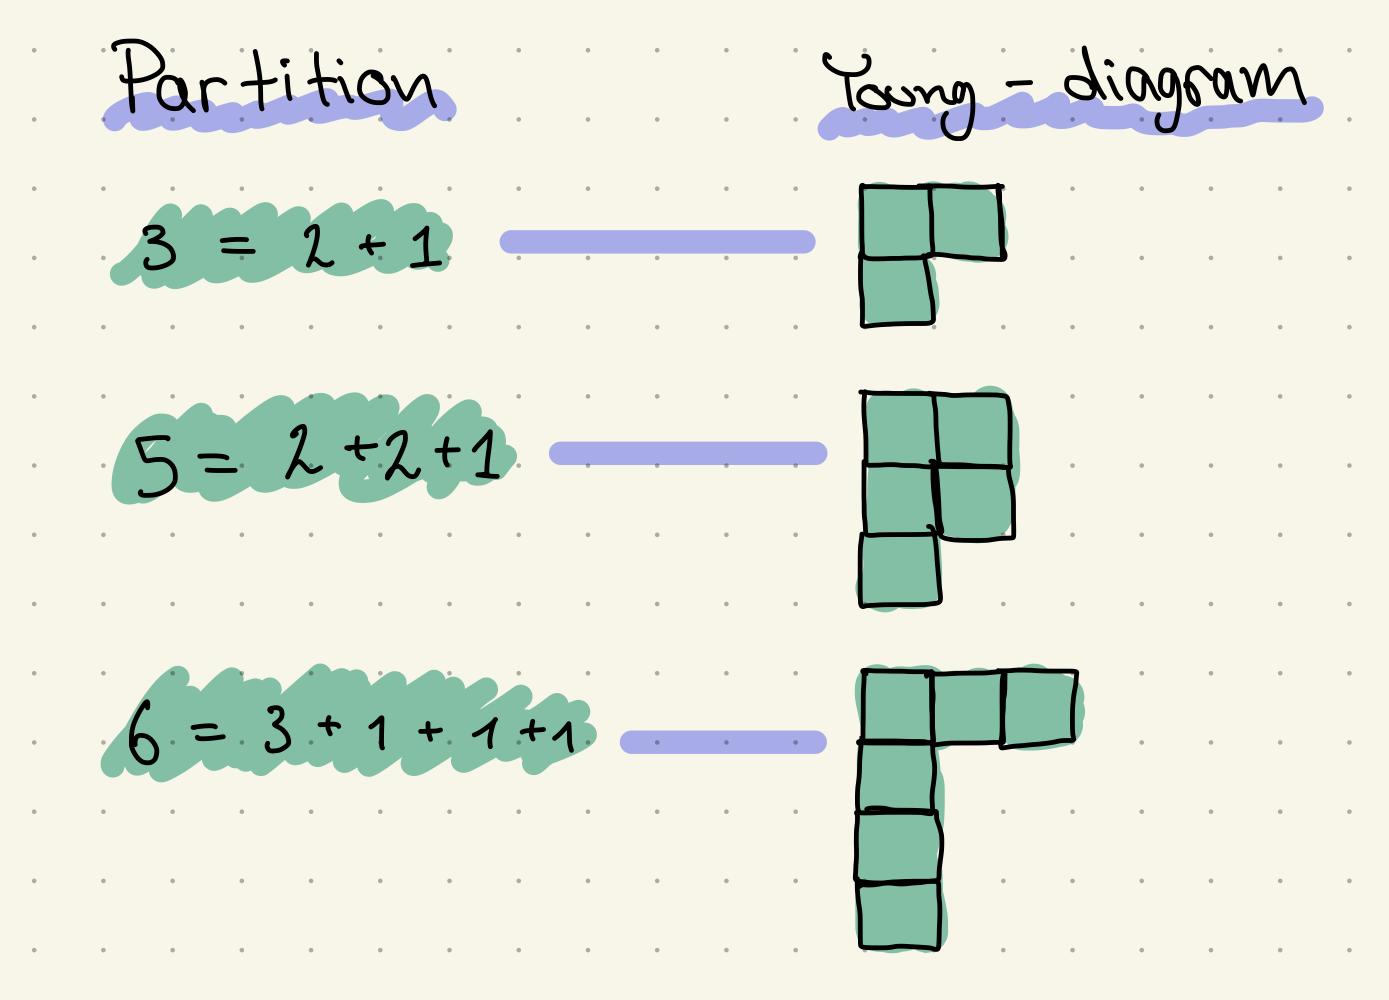
\includegraphics[width=8cm]{youngdiagram.jpeg}
        \caption{Examples for young diagrams associated to partitions.}
    \end{figure}
\end{defi}
One easily checks that partitions of an integer $k$ correspond one-to-one to
Young diagrams with $k$ boxes.
There is an involution on the set of Young diagrams, given by \emph{transposing}
the diagram. This yields an involution on the set of partitions.
\begin{defi}[Transpose partition]
    Given a partition $\lambda = (l_1 \geq l_2 \geq \dots \geq l_r)$, the 
    \emph{transpose partition} is given by $\lambda^\dagger = 
    (l^\dagger_1 \geq l^\dagger_2 \geq \dots \geq l^\dagger_s)$, where
    \begin{equation*}
        l^\dagger_i = \# \{j \mid l_j \geq i\}.
    \end{equation*}
    In particular, we find $s = l_1$.
    This definition makes much more sense in terms of Young diagrams.
    \begin{figure}[H]
        \centering
        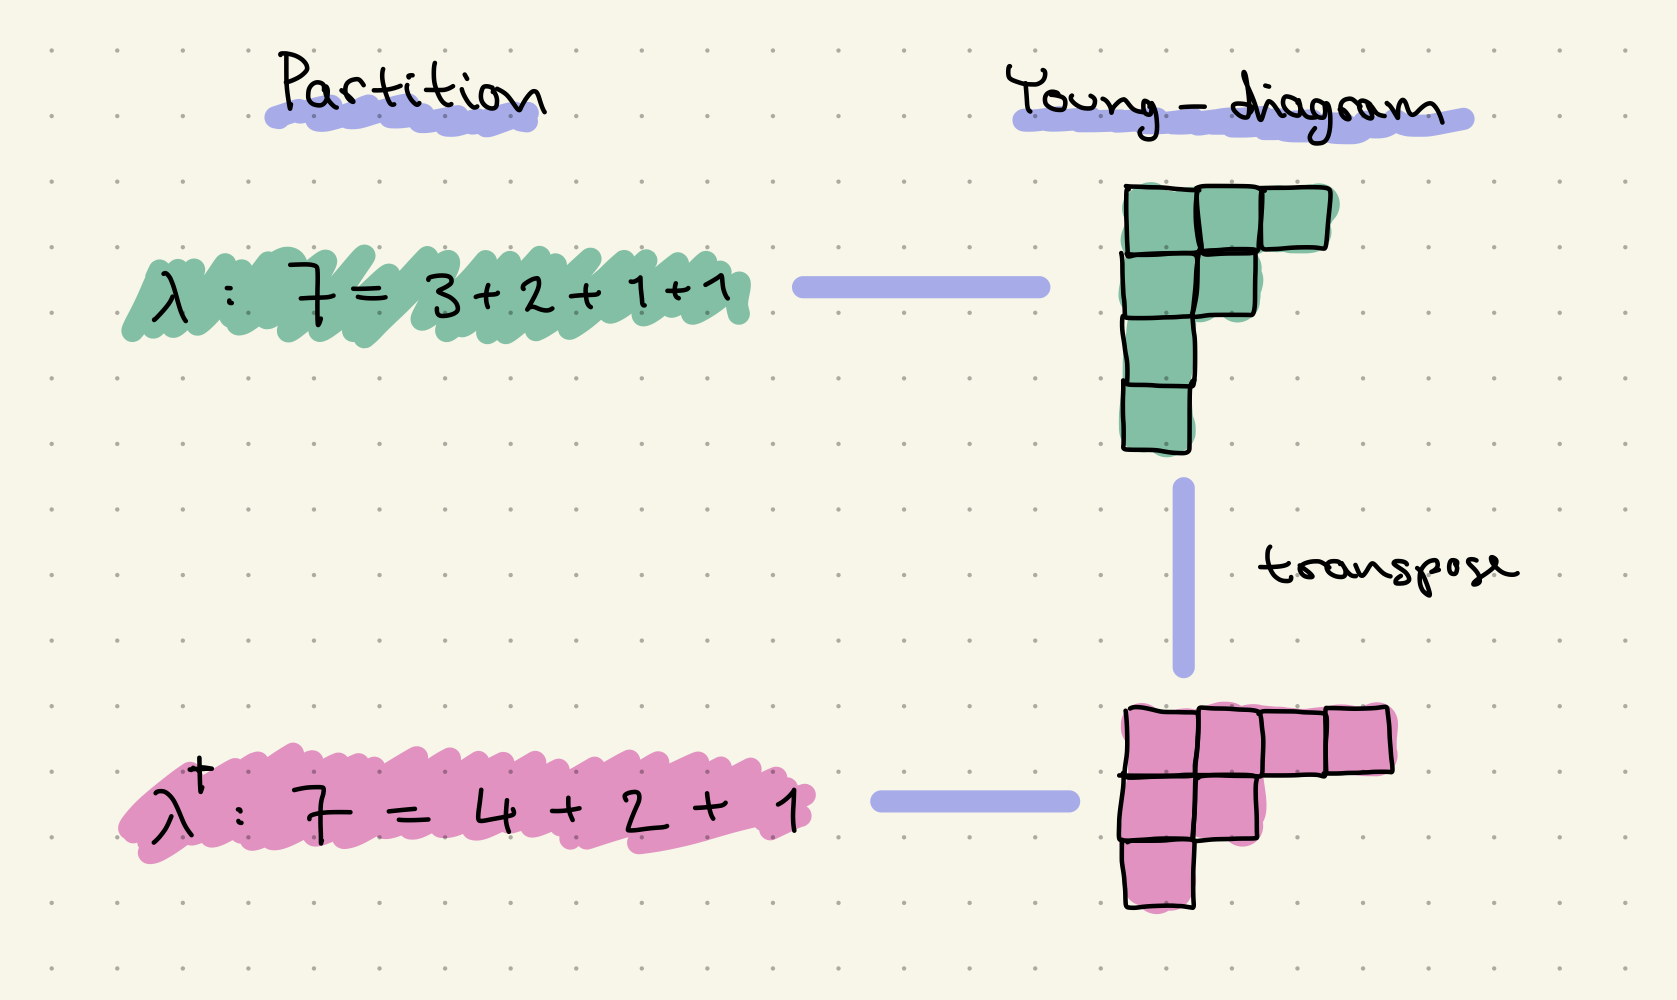
\includegraphics[width=10cm]{transpose.jpeg}
        \caption{Example of a transpose partition}
    \end{figure}
\end{defi}


We care about partitions because they are in natural (whatever this means here)
bijection with the "fundamental building blocks" of $\GPoly$.

\begin{thm}[Structure of $\GPoly$, \cite{macdonald1998symmetric}, \cite{sam2012introduction}]
    The category $\GPoly$ is an abelian and semisimple tensor category. The
    simple objects are indexed
    by partitions: For each integer $k$ and each partition $\lambda$ of $k$, there 
    is a \emph{Schur-functor} $S_\lambda$, which is a homogenous polynomial functor
    of degree $k$.
\end{thm}
In practice, this means that any graded polynomial functor $F$ can uniquely be written as
\begin{equation*}
    F = \bigoplus_{k \in \N} \bigoplus_{\lambda \pof k} S_\lambda^{\oplus a_\lambda}.
\end{equation*}
\textbf{Remark.} Categories with this structure seem to appear a lot. For
example, the category of $S_*$-representations (with objects $(V_n)_{n \in \N}$, where
$V_n$ is a representation of $S_n$) is equivalent to $\GPoly$. For more on this,
see \cite{sam2012introduction}.

The reason this is interesting for us is that the functors $\Sym^k$ and
$\bigwedge{}^k$ are Schur-functors! 
Even better, the functor $\Sym^k$ belongs to the partition $(k)$, the functor
$\bigwedge{}^k$ belongs to $(1,\dots, 1)$. These partitions are mutual transpose 
of one another, which is a deep connection between $\Sym$ and $\bigwedge$, a lot 
deeper than the list of similarities we found before.

One might hope that transposition of partitions somehow descents to 
a transposition operation on $\GPoly$. This hope is fulfilled!
\begin{thm}[]
    There is an additive endofunctor $\Omega: \GPoly \to \GPoly$ such that 
    $\Omega(S_\lambda) = S_{\lambda^\dagger}$.
\end{thm}
One construction of this functor can be found in Gandini's paper,
\cite{Gandini2019ResOfIdeals}, but there are many interesting remarks in
\cite{sam2012introduction}. In this last paper, the authors show that $\Omega$
is even an equivalence of symmetric monoidal categories. In particular, 
it is exact and preserves module- and algebra objects. Remember that we want to
prove that the ideal $I'(\cA_G) = \cI'_{\cA_G}(K)$ is generated in degree $\leq
\#G$. We know the corresponding statement for $I(\cA_G)$, and Gandini shows
that we only have to apply $\Omega$ in order to obtain the statement for
$I'(\cA_G)$:
\begin{prop}(\cite[Proposition 6.1]{Gandini2019ResOfIdeals})
    If $\cR \in \GPoly$ is an algebra object and $\cM$ is a $\cR$-module object
    "of regularity $\leq t$",\footnote{Again, this needs a suitable adaptation of \emph{regularity} in this setting. We won't go into this here.} then $\Omega(\cM)(V)$ is generated in degree 
    $\leq t$ over $\cR(V)$ for every $V \in \FinVec$. 
\end{prop}
Here again we couldn't get around \textit{regularity}. We need a final lemma to
conclude.
\begin{lem}
    We have $\Omega(\cI_\cA) \cong \cI'_\cA$.
\end{lem}
\begin{proof}
    \red{I didn't find a proof of this, Gandini simply uses this statement in 
    \cite{gandini2021degree}. Perhaps we can write $\cI_\cA$ and 
    $\cI_\cA'$ as some Kernels that get mapped into one another.}
\end{proof}

It can be shows that the functor $\cI_{\cA}$ is of regularity $\leq t$ if
$\cA$ is a subspace arrangement of $t$ subspaces. Using the previous two 
results, this shows that $I'(\cA) = \cI'_{\cA}(K)$ is generated over $\bigwedge(V)$
in degree $\leq t$. Applying this result to the subspace arrangement 
associated with the action of $G$ on $V$, we obtain Theorem \ref{thm:newcrux}.
This concludes the proof of the subspace arrangement theorem, which also
finishes the proof of Noether's degree bound for the exterior algebra.
\end{document}
